\subsection{Slučaj upotrebe: Objavljivanje rezultata}

\subsubsection*{Kratak opis}
Izborna komisija objavljuje rezultate završenih izbora ili, ukoliko nije ispunjen uslov minimalne izlaznosti, obaveštenje o potrebi ponavljanja izbora.

\subsubsection*{Akteri}
\begin{itemize}
    \item \textbf{Član izborne komisije} -- pregleda izlaznost i rezultate i potvrđuje njihovo objavljivanje.
\end{itemize}

\subsubsection*{Preduslovi}
\begin{itemize}
    \item Član izborne komisije je prijavljen u sistem.
    \item Period glasanja je završen.
    \item Sistem je evidentirao i prebrojao glasove.
\end{itemize}

\subsubsection*{Postuslovi}
\begin{itemize}
    \item Ako je izlaznost veća ili jednaka 50\% i komisija potvrdi objavljivanje, rezultati postaju dostupni studentima.
    \item Ako je izlaznost manja od 50\% i komisija potvrdi objavljivanje obaveštenja, studenti dobijaju informaciju da se izbori ponavljaju.
    \item Ako komisija odustane od objavljivanja, status izbora ostaje nepromenjen.
\end{itemize}

\subsubsection*{Osnovni tok}
\begin{enumerate}
    \item Član komisije bira opciju \textbf{Pregled rezultata}.
    \item Sistem prikazuje broj studenata sa pravom glasa, broj studenata koji su glasali i procenat izlaznosti.
    \item Sistem proverava da li je izlaznost veća ili jednaka 50\%.
    \item Ako je uslov ispunjen, sistem prikazuje rezultate glasanja, odnosno broj glasova koji je dobila svaka izborna lista.
    \item Član komisije pregleda rezultate.
    \item Član komisije bira opciju \textbf{Objavi}.
    \item Sistem objavljuje rezultate i prikazuje poruku o uspešnom objavljivanju.
\end{enumerate}

\subsubsection*{Alternativni tokovi}
\begin{enumerate}[label=\textbf{A\arabic*.}]
    \item \textbf{Izlaznost je manja od 50\%.} Sistem u koraku 3 prikazuje obaveštenje da izbori nisu važeći. Član komisije bira opciju za objavljivanje obaveštenja o ponavljanju izbora. Sistem objavljuje obaveštenje koje je dostupno studentima, a rezultati se ne objavljuju kao važeći. Slučaj upotrebe se završava.
    \item \textbf{Odustajanje od objavljivanja.} Ako član komisije ne potvrdi objavljivanje, sistem ne objavljuje ni rezultate ni obaveštenje. Komisija kasnije može ponovo da pristupi ovoj funkcionalnosti.
\end{enumerate}

\begin{figure}[H]
    \centering
    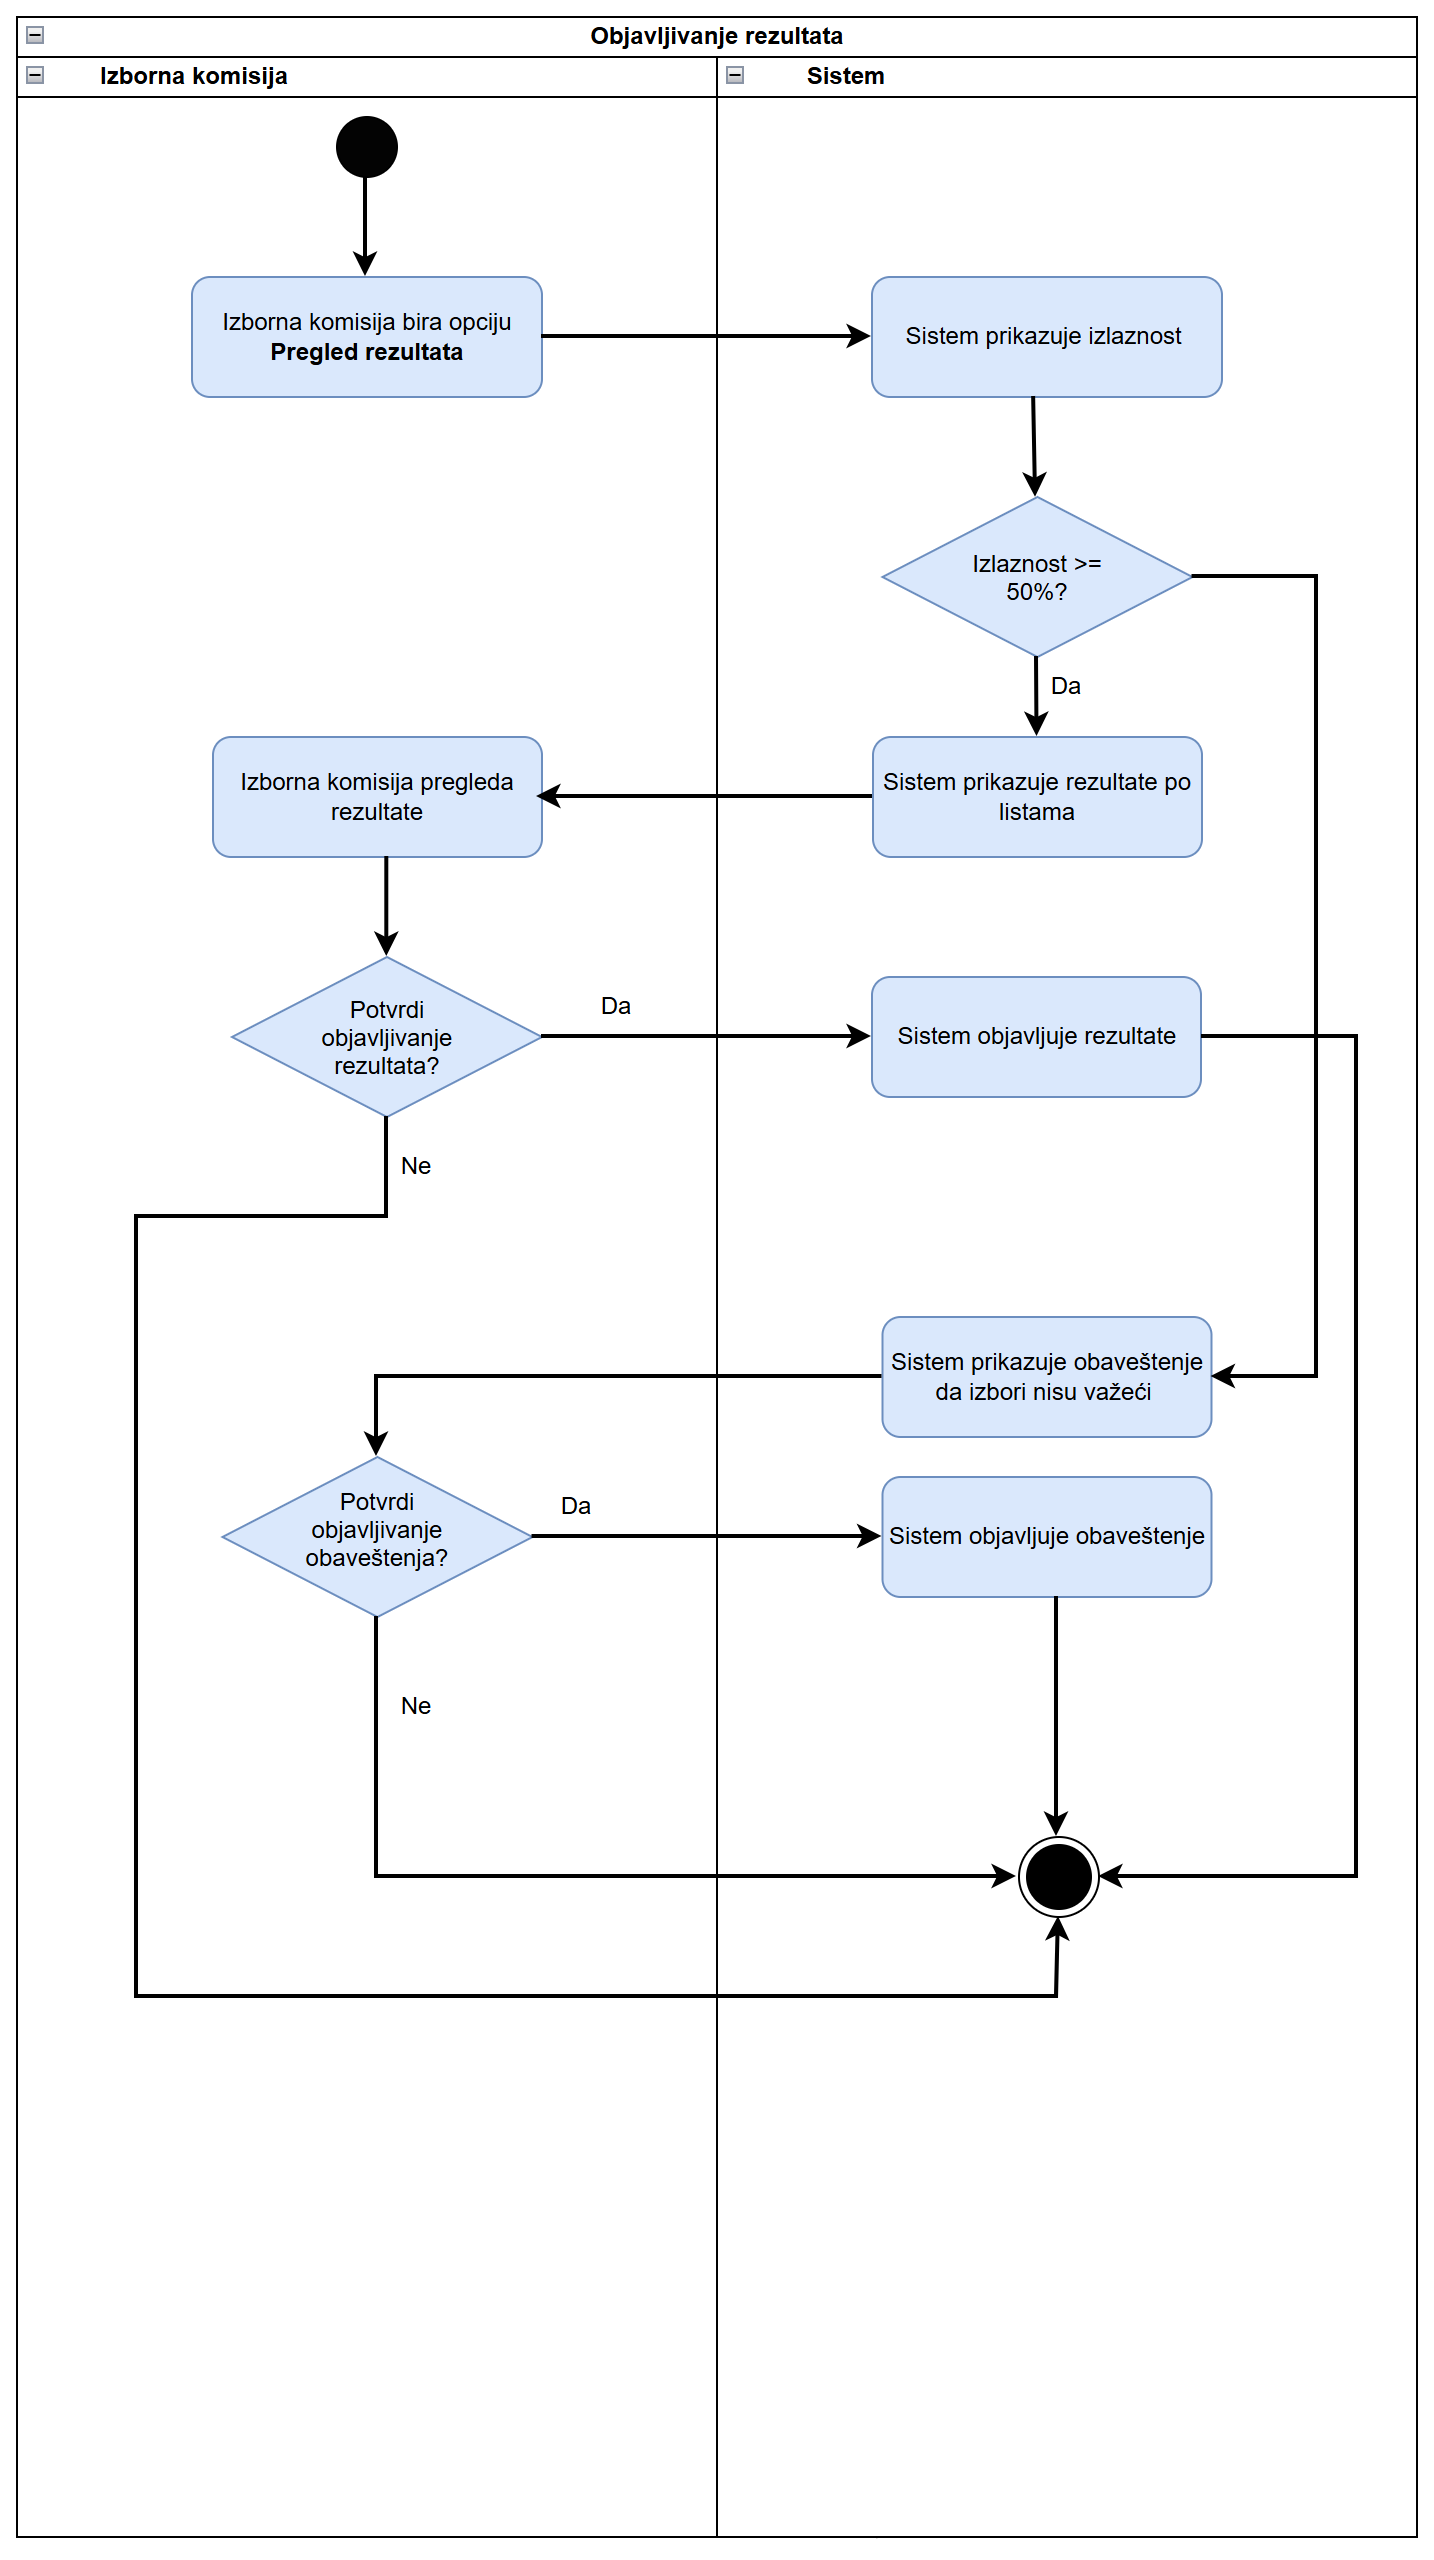
\includegraphics[height=0.8\textheight]{objavljivanje_rezultata.png}
    \caption{Dijagram aktivnosti: Objavljivanje rezultata}
    \label{fig:objavljivanje_rezultata}
\end{figure}

\begin{figure}[H]
    \centering
    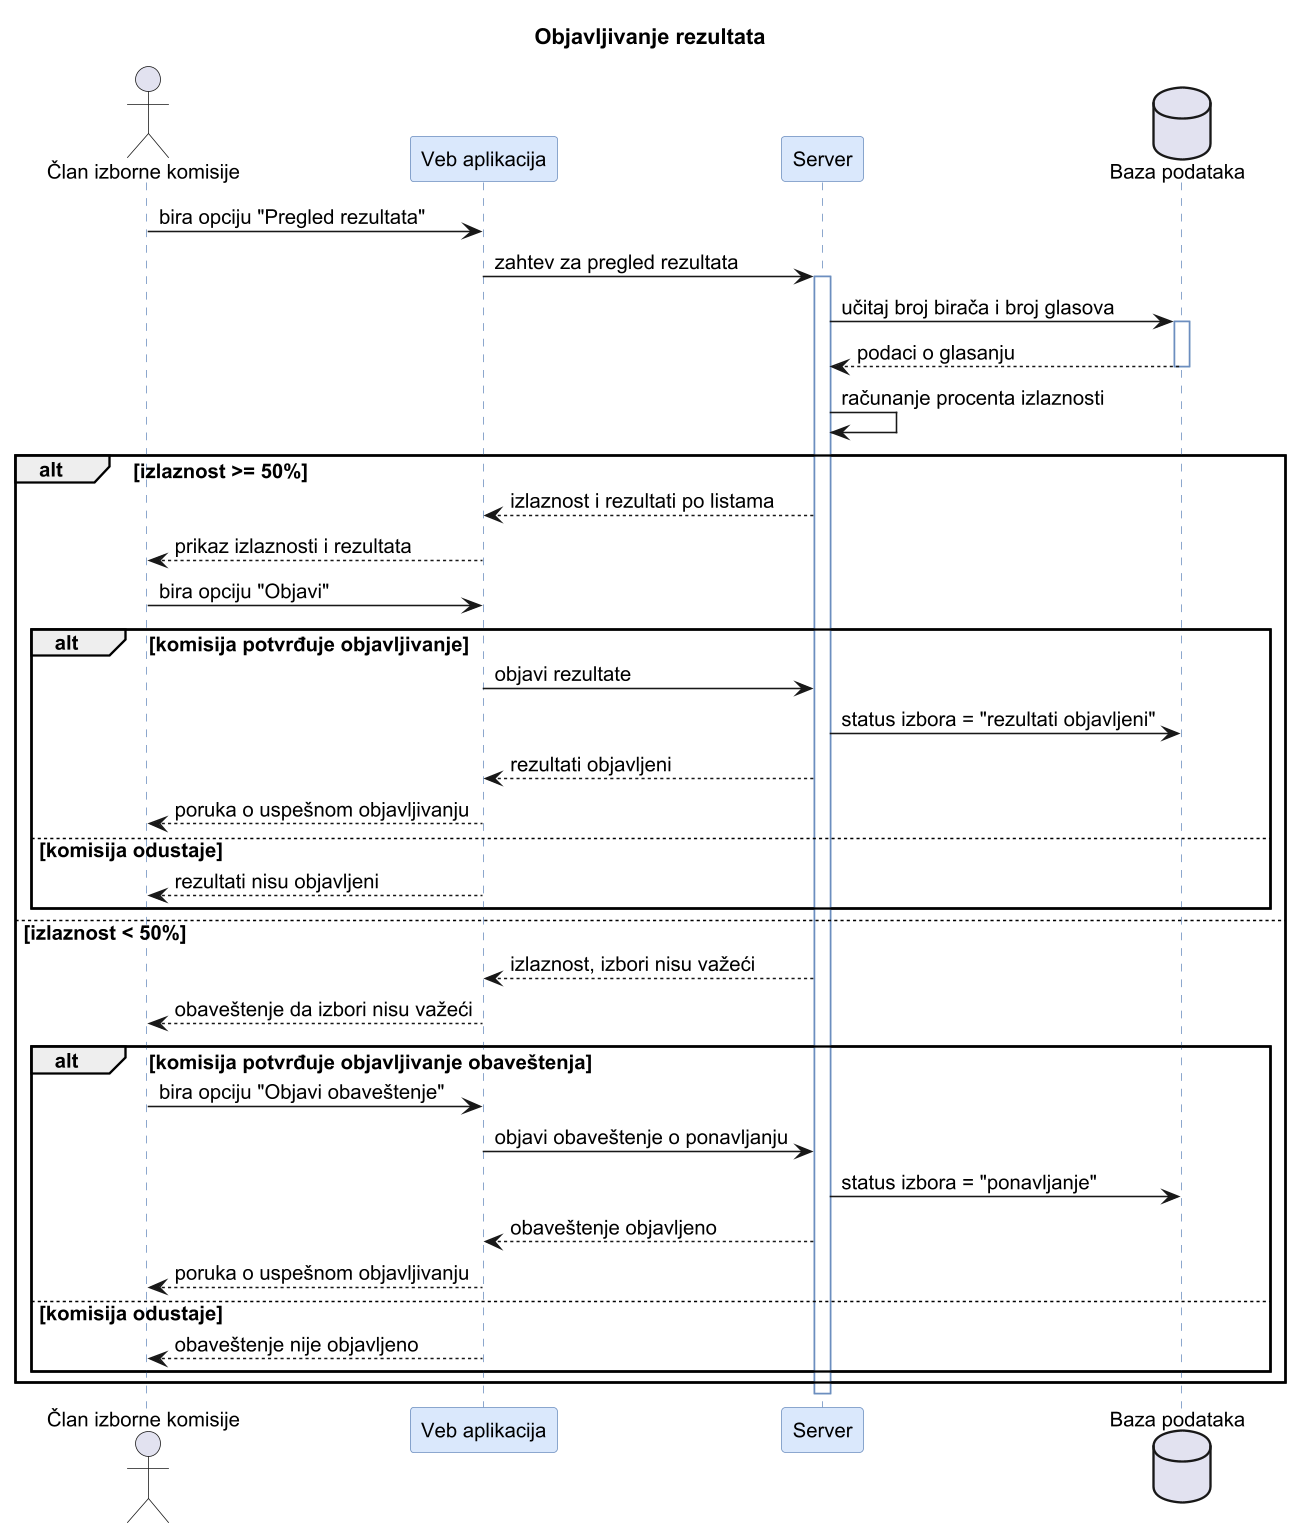
\includegraphics[width=\textwidth,height=0.8\textheight,keepaspectratio]{sekvenca_objavljivanje_rezultata.png}
    \caption{Dijagram sekvence: Objavljivanje rezultata}
    \label{fig:sekvenca_objavljivanje_rezultata}
\end{figure}

\newpage
